%----------------------------------------------------------
% Number of pages for Synopsis: 5 to 10
% All Rights Reserved @Prof.Vishal Badgujar
% Information Technology Department 
% A.P.Shah Institute of Technology, Thane
%----------------------------------------------------------
% List of command to convert synopsis.tex to synopsis.pdf
%----------------------------------------------------------
%pdflatex synopsis.tex
%evince synopsis.pdf &
\documentclass[12pt,singleside,a4paper]{article}
\usepackage{epsfig}
\usepackage{cite}
\usepackage{geometry}
\geometry{left=20mm,right=20mm,top=20mm,bottom=50mm}
\pagestyle{plain}
\begin{document}
\pagenumbering{arabic}
\begin{titlepage}
\vspace*{0.25cm}
{\centering
{\Large\textbf {Eye Control System Based on Hough Transform
Algorithm}}\\
\vspace{1cm}
 Submitted in partial fulfillment of the requirements\\
of the degree of\\ \vspace{1cm}
{\large\textbf {Bachelor of Engineering}}\\
\vspace{0.5cm}
in \\
\vspace{0.5cm}
{\large\textbf {Computer Science}}\\
\vspace{0.5cm}
by\\
\vspace{0.5cm}

{\large \textbf {Anindita Chowdhury}} {\large \textbf {(15102067)}}\\
\vspace{0.2cm}
{\large \textbf {Anamika Sonavane}} {\large \textbf {(15102018)}}\\
\vspace{0.2cm}
{\large \textbf {Vibha Gaikwad}} {\large \textbf {(16202014)}}\\
\vspace{1cm}

Guide \\ 
\vspace{0.3cm}

\hspace{.05cm} {\large \textbf {Prof. Sachin Takmare}}\\
\vspace{1.5cm}
\begin{figure}[h]
\centering

\includegraphics[scale=0.30]{apsit_logo.jpg}
\end{figure}

\hspace{.05cm}
\hspace{.05cm}

{\textbf {Department of Computer Engineering}}\\
A.P. Shah Institute of Technology\\
G.B.Road,Kasarvadavli, Thane(W), Mumbai-400615\\
UNIVERSITY OF MUMBAI\\
2017-2018\\}
\end{titlepage}
\newpage
\thispagestyle{empty}
\vspace*{0.2cm}
\vspace{1cm}
\begin{center}
 \large\textbf{CERTIFICATE}
\end{center}
\vspace{1cm}


\par This is to certify that the project Synopsis entitled \textbf{\textit{``Eye Control System Based on Hough Transform
Algorithm"}} is a bonafide work of \textbf{\textit{``Anindita Chowdhury (15102067), Anamika Sonavane (15102018), Vibha Gaikwad (16202014)"}}  submitted to the University of Mumbai in partial fulfillment of the requirement for the award of the degree of \textbf{\textit{Bachelor of Engineering} }in\textbf{ \textit{Computer Science.}}\\

\vspace{30mm}
%\hfill
\begin{tabular}{@{}l@{}}
\hspace{3mm}(Prof. Sachin Takmare)\hspace{78mm}         \\
\hspace{3mm}   Guide \hspace{95mm}               \\
%\vspace{5mm}\\
\end{tabular}


%\vspace{5mm}\\

\vspace{30mm}
%\hfill
\begin{tabular}{@{}l@{}}
External Examiner	 \hspace{62mm}        Prof.Sachin H. Malave \\
 \hspace{98mm}             Head Of Department\\

%\vspace{5mm}\\
\end{tabular}

\vspace{30mm}
%\hfill
\begin{tabular}{@{}l@{}}
 \hspace{61mm}        Dr. Uttam. D. Kolekar  \\
   \hspace{76mm}             Principal\\

%\vspace{5mm}\\
\end{tabular}




\vspace{5mm}


















\pagebreak
\section*{Abstract}
\hspace{1mm} These days the lifestyle and living of the world has changed a lot, Technology plays a very important part in one’s life. Thus,this paper proposes an eye control system employing eye gaze tracking techniques that might be helpful for those limb disabled people with healthy eyes. We design a motion function as well as an efficiently blink detection function. With these functions, users can select any button, link or can move the mouse anywhere on the screen, with their eyes only, through a conventional camera mounted on top of the computer or laptop. Digital Image Processing here will be used to process the image, with the help of hough transform algorithm, which will initially help us capture the image of eye, process the images into templates and creating a database which will be further used to compare with the real time images.

%------------------------------
\section*{Introduction}
\hspace{1mm}More than 1 billion people in the world have some form of disability. This corresponds to about 15\% of the world's population.Census 2001 has revealed that over 21 million people in India are suffering from one or the other kind of disability. This is equivalent to 2.1\% of the population.Now in this population some are limb-disabled. Although this number is very small, but it matters to those who can not enjoy the digital world.\vspace{2mm}\newline
Due to their limb handicap, such vast amount of people cannot enjoy the convenience and entertainment of the ever advancing computer technology. A person's eyes convey a great deal of information with regards to the meaning behind certain facial expressions. Also, the direction in which an individual is looking shows where his or her attention is focused. By tracking the position of the iris, useful interfaces can be developed that allow the user to control and manipulate devices in a more natural manner. So, this paper has purpose of meeting the specific needs of these limb disabled people.
\section*{Objectives}
Objectives of this project are:
\newline
\begin{itemize}

\item To design a system that controls mouse actions using Eye-Tracking.

\item To design an effective system that enables limb-disabled people with healthy eyes to use computer.

\item To eliminate use of any external Head-Mounted Eye Tracker and replace it with a normal camera. 

\end{itemize}
\newpage
\section*{Literature Review}
Eye-tracking experiments have an early history. One of the earliest eye-trackers was designed by Edmund Huey (Huey, 1908) which just consisted of a contact lens like device with a hole for the pupil.\vspace{2mm}\newline
Generally, eye tracking measures the eyeball position and determines gaze direction of a person, and the movements of the eye can be tracked using different technologies. It can be categorized into four categories: infrared-oculography (IROG), scleral search coil method (SSC), electrooculography (EOG), and video-oculography (VOG). Currently, most of the eye tracking researches for HCI are based on VOG, because the VOG technique has minimized the invasiveness to user in some degree.\vspace{2mm}\newline
Eye-tracking has found its applications in many projects. In 2006 a group of Taiwanese engineers developed a "Powered Wheelchair controlled by Eye-Tracking system". In 2016 conducted a comparative study of user experience in online-social media branding web pages using eye-tracker.

\section*{Problem Definition}
\par This project uses eye gaze position and eye-state (starring or blinking) for enabling virtual mouse, so as to make it possible for limb-disabled people to experience the digital world. The camera will capture image frames of eye pupil as input. After  the eye is detected it will be processed for calibration. Processing should include conversion to gray-scale followed by canny-edge detection , which will be used to detect pupil center using Hough transform algorithm.\vspace{2mm}\newline
The user can gaze any where on the screen and for selecting a link / clicking a button, the user must blink. If the blink duration exceeds 2 seconds, the it will be considered as a click, otherwise not. Instead of using additional head mounted eye-tracker , the laptop camera will be used. If the camera is inefficient, then external camera, connected to the computer via USB cable or bluetooth should be used.
\pagebreak
%
%\begin{figure}[h]
%\begin{center}
%\scalebox{0.25}{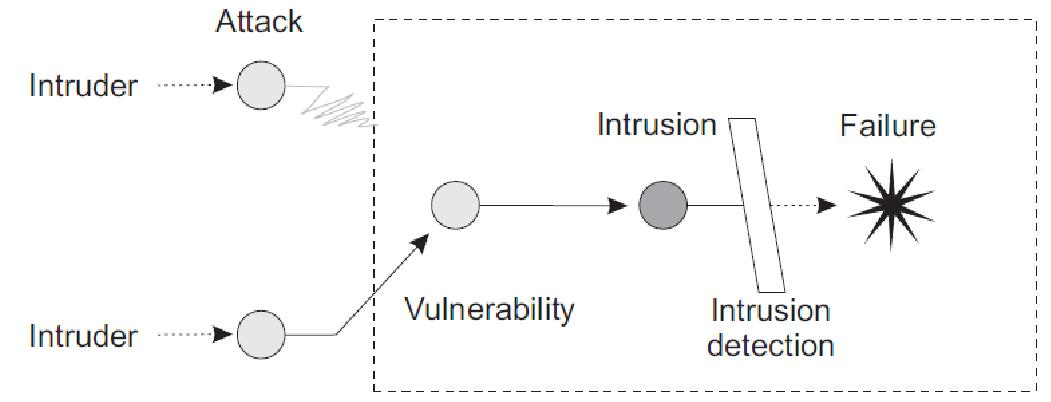
\includegraphics{1.jpg}}
%\end{center}
%\caption {Intrusion Detection System}
%\label{IDS}
%\vspace{0mm}
%\end{figure}
%
\section*{Proposed System Architecture/Working}
\vspace{0.1mm}
%
\begin{figure}[h]
\begin{center}
\scalebox{0.42}{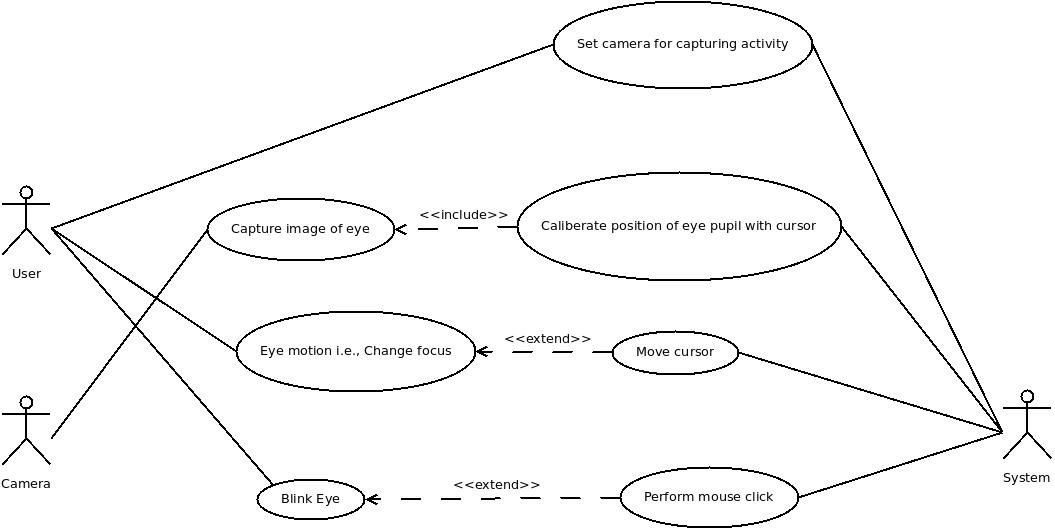
\includegraphics{use-case-diagram.jpeg}}
\caption {Use case diagram}
\label{IDS}
\vspace*{\floatsep}
\scalebox{0.8}{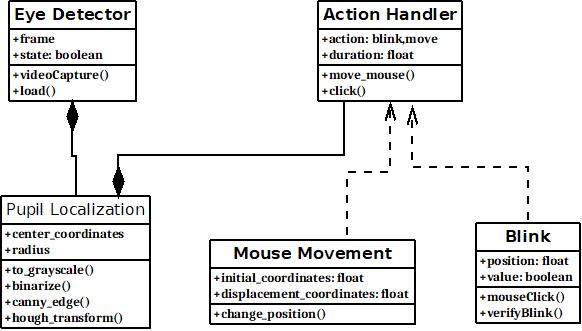
\includegraphics{class-diagram.jpg}}
\end{center}
\caption {Class diagram}
\label{IDS}
\end{figure}
%

\newpage
\section*{Summary}
The work presented in this report is related to Eye-tracking System. This paper designs an eye control system using the gaze method, the ameliorated Hough transform algorithm and an efficient blink detection method, with the purpose of meeting the specific needs of disabled people with healthy eyes. In order to make user interact with computer naturally and conveniently by only using their eye, we provide an eye tracking based control system. Although, some aspects are needed to be guaranteed; one important aspect is the lighting conditions, second is face and eye illumination, which should be homogenous most natural possible.
%\pagebreak 

\begin{thebibliography}{}
\addcontentsline{toc}{chapter}{Bibliography}

\bibitem{bm}
``Real Time Eye Gaze Controlled Human Computer  Interface for Paralyzed People", http://www.ijsrd.com/articles/IJSRDV4I10907.pdf, January 2016


\bibitem{bm}
``A Survey on Eye Tracking and Detection",\newline
https://www.ijirset.com/upload/2015/coctoer/76\_A\_Survey.pdf, Octoer 10, 2015


\bibitem{bm}
``Literature Survey on Eye-Tracking", http://www.cfilt.iitb.ac.in/resources/surveys/eye-tracking-nivvedan-may14.pdf, May 2014


\bibitem{bm}
``DESIGN AND IMPLEMENTATION OF A HUMAN COMPUTER INTERFACE TRACKING SYSTEM BASED ON MULTIPLE EYE FEATURES" , http://www.jatit.org/volumes/research-papers/Vol9No2/8Vol9No2.pdf


\bibitem{bm}
``Eye Control System Base on Ameliorated Hough Transform Algorithm" , https://ieeexplore.ieee.org/document/6516004/, September 9, 2013


\end{thebibliography}
\newpage

\section{Publication}

Paper entitled \textbf{``Paper Title"} is presented at \textbf{``International Conference/Journal Name"} by \textbf{``Author Name".}\\


\end{document} 
 
